\documentclass{article}
% All LaTeX documents including
% tikz() output must use this
% package!
\usepackage{tikz}
\usepackage{multirow}
\usepackage{graphicx}
\usepackage[top=0.5cm, bottom=0.5cm, outer=0.5cm, inner=0.5cm, heightrounded,
  marginparwidth=0.5cm, marginparsep=0.2cm]{geometry}
\begin{document}
\begin{figure}[!h]
\centering
    \begin{tabular}{| l | *{3}{r} | c c c |}
      \hline
      \multirow{1}{*}Threads & gnparser & gbif-parser & biodiversity
      & \multicolumn{3}{c |}{Ratio} \\
      \cline{5-7}
      & & & & gn & gbif & bio \\
      \hline
      1  & 8178  & 6389  & 1111 & 1 & 0.78 & 0.14 \\
      2  & 14125 & 12638 & 1722 & 1 & 0.89 & 0.12 \\
      4  & 25125 & 21994 & 2556 & 1 & 0.88 & 0.10 \\
      8  & 33541 & 30972 & 2777 & 1 & 0.92 & 0.08 \\
      12 & 36369 & 31833 & 2527 & 1 & 0.88 & 0.07 \\
      \hline
    \end{tabular}
    % Created by tikzDevice version 0.10.1 on 2016-06-02 07:38:12
% !TEX encoding = UTF-8 Unicode
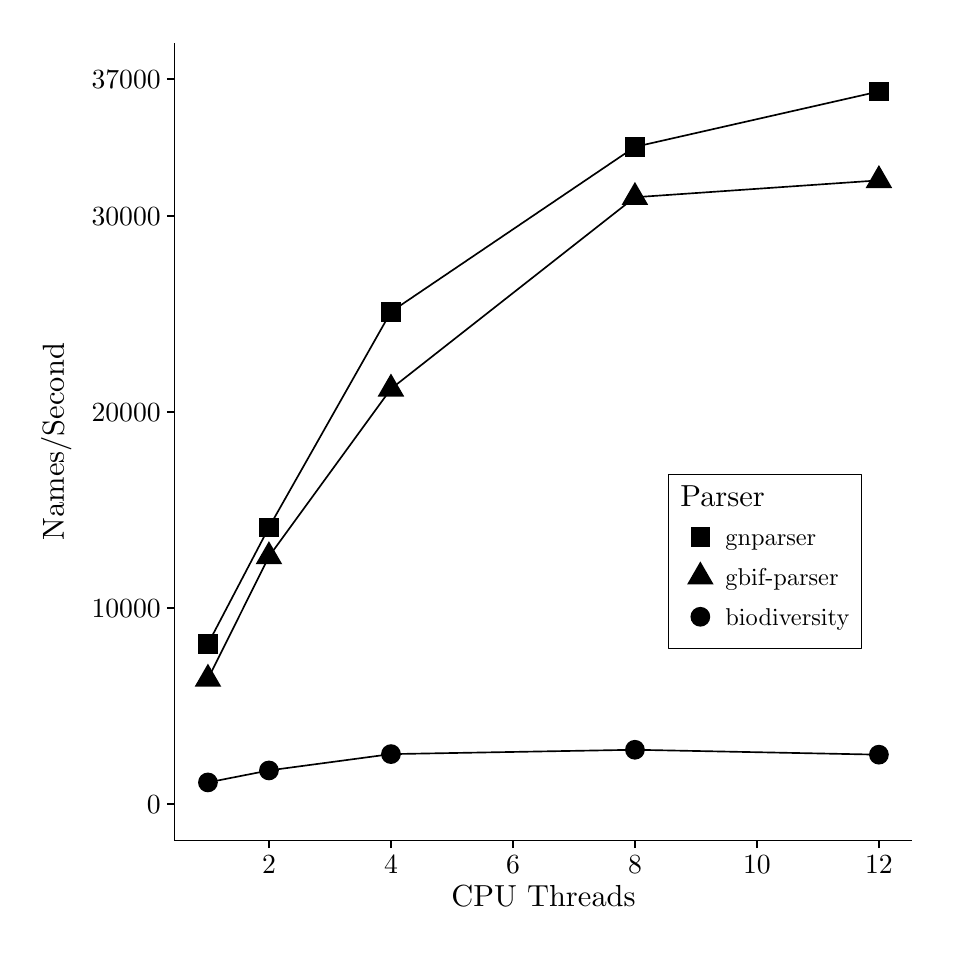
\begin{tikzpicture}[x=1pt,y=1pt]
\definecolor{fillColor}{RGB}{255,255,255}
\path[use as bounding box,fill=fillColor,fill opacity=0.00] (0,0) rectangle (325.21,325.21);
\begin{scope}
\path[clip] (  0.00,  0.00) rectangle (325.21,325.21);
\definecolor{drawColor}{RGB}{255,255,255}
\definecolor{fillColor}{RGB}{255,255,255}

\path[draw=drawColor,line width= 0.6pt,line join=round,line cap=round,fill=fillColor] (  0.00,  0.00) rectangle (325.21,325.21);
\end{scope}
\begin{scope}
\path[clip] ( 53.02, 31.51) rectangle (319.71,319.71);
\definecolor{fillColor}{RGB}{255,255,255}

\path[fill=fillColor] ( 53.02, 31.51) rectangle (319.71,319.71);
\definecolor{drawColor}{RGB}{255,255,255}

\path[draw=drawColor,line width= 0.3pt,line join=round] ( 53.02, 80.02) --
	(319.71, 80.02);

\path[draw=drawColor,line width= 0.3pt,line join=round] ( 53.02,150.83) --
	(319.71,150.83);

\path[draw=drawColor,line width= 0.3pt,line join=round] ( 53.02,221.64) --
	(319.71,221.64);

\path[draw=drawColor,line width= 0.3pt,line join=round] ( 53.02,281.83) --
	(319.71,281.83);

\path[draw=drawColor,line width= 0.3pt,line join=round] ( 65.14, 31.51) --
	( 65.14,319.71);

\path[draw=drawColor,line width= 0.3pt,line join=round] (109.22, 31.51) --
	(109.22,319.71);

\path[draw=drawColor,line width= 0.3pt,line join=round] (153.31, 31.51) --
	(153.31,319.71);

\path[draw=drawColor,line width= 0.3pt,line join=round] (197.39, 31.51) --
	(197.39,319.71);

\path[draw=drawColor,line width= 0.3pt,line join=round] (241.47, 31.51) --
	(241.47,319.71);

\path[draw=drawColor,line width= 0.3pt,line join=round] (285.55, 31.51) --
	(285.55,319.71);

\path[draw=drawColor,line width= 0.6pt,line join=round] ( 53.02, 44.61) --
	(319.71, 44.61);

\path[draw=drawColor,line width= 0.6pt,line join=round] ( 53.02,115.42) --
	(319.71,115.42);

\path[draw=drawColor,line width= 0.6pt,line join=round] ( 53.02,186.24) --
	(319.71,186.24);

\path[draw=drawColor,line width= 0.6pt,line join=round] ( 53.02,257.05) --
	(319.71,257.05);

\path[draw=drawColor,line width= 0.6pt,line join=round] ( 53.02,306.61) --
	(319.71,306.61);

\path[draw=drawColor,line width= 0.6pt,line join=round] ( 87.18, 31.51) --
	( 87.18,319.71);

\path[draw=drawColor,line width= 0.6pt,line join=round] (131.27, 31.51) --
	(131.27,319.71);

\path[draw=drawColor,line width= 0.6pt,line join=round] (175.35, 31.51) --
	(175.35,319.71);

\path[draw=drawColor,line width= 0.6pt,line join=round] (219.43, 31.51) --
	(219.43,319.71);

\path[draw=drawColor,line width= 0.6pt,line join=round] (263.51, 31.51) --
	(263.51,319.71);

\path[draw=drawColor,line width= 0.6pt,line join=round] (307.59, 31.51) --
	(307.59,319.71);
\definecolor{drawColor}{RGB}{0,0,0}

\path[draw=drawColor,line width= 0.6pt,line join=round] ( 65.14, 52.48) --
	( 87.18, 56.81) --
	(131.27, 62.71) --
	(219.43, 64.28) --
	(307.59, 62.51);

\path[draw=drawColor,line width= 0.6pt,line join=round] ( 65.14, 89.85) --
	( 87.18,134.11) --
	(131.27,194.69) --
	(219.43,263.93) --
	(307.59,270.03);

\path[draw=drawColor,line width= 0.6pt,line join=round] ( 65.14,102.52) --
	( 87.18,144.63) --
	(131.27,222.53) --
	(219.43,282.13) --
	(307.59,302.15);
\definecolor{fillColor}{RGB}{0,0,0}

\path[fill=fillColor] ( 61.57, 98.95) --
	( 68.71, 98.95) --
	( 68.71,106.09) --
	( 61.57,106.09) --
	cycle;

\path[fill=fillColor] ( 83.61,141.07) --
	( 90.75,141.07) --
	( 90.75,148.20) --
	( 83.61,148.20) --
	cycle;

\path[fill=fillColor] (127.70,218.96) --
	(134.83,218.96) --
	(134.83,226.10) --
	(127.70,226.10) --
	cycle;

\path[fill=fillColor] (215.86,278.56) --
	(223.00,278.56) --
	(223.00,285.69) --
	(215.86,285.69) --
	cycle;

\path[fill=fillColor] (304.02,298.58) --
	(311.16,298.58) --
	(311.16,305.72) --
	(304.02,305.72) --
	cycle;

\path[fill=fillColor] ( 65.14, 95.40) --
	( 69.95, 87.08) --
	( 60.34, 87.08) --
	cycle;

\path[fill=fillColor] ( 87.18,139.66) --
	( 91.99,131.34) --
	( 82.38,131.34) --
	cycle;

\path[fill=fillColor] (131.27,200.24) --
	(136.07,191.92) --
	(126.46,191.92) --
	cycle;

\path[fill=fillColor] (219.43,269.48) --
	(224.23,261.16) --
	(214.62,261.16) --
	cycle;

\path[fill=fillColor] (307.59,275.58) --
	(312.40,267.25) --
	(302.79,267.25) --
	cycle;

\path[fill=fillColor] ( 65.14, 52.48) circle (  3.57);

\path[fill=fillColor] ( 87.18, 56.81) circle (  3.57);

\path[fill=fillColor] (131.27, 62.71) circle (  3.57);

\path[fill=fillColor] (219.43, 64.28) circle (  3.57);

\path[fill=fillColor] (307.59, 62.51) circle (  3.57);
\end{scope}
\begin{scope}
\path[clip] (  0.00,  0.00) rectangle (325.21,325.21);
\definecolor{drawColor}{RGB}{0,0,0}

\path[draw=drawColor,line width= 0.6pt,line join=round] ( 53.02, 31.51) --
	( 53.02,319.71);
\end{scope}
\begin{scope}
\path[clip] (  0.00,  0.00) rectangle (325.21,325.21);
\definecolor{drawColor}{RGB}{0,0,0}

\node[text=drawColor,anchor=base east,inner sep=0pt, outer sep=0pt, scale=  1.00] at ( 48.07, 41.17) {0};

\node[text=drawColor,anchor=base east,inner sep=0pt, outer sep=0pt, scale=  1.00] at ( 48.07,111.98) {10000};

\node[text=drawColor,anchor=base east,inner sep=0pt, outer sep=0pt, scale=  1.00] at ( 48.07,182.79) {20000};

\node[text=drawColor,anchor=base east,inner sep=0pt, outer sep=0pt, scale=  1.00] at ( 48.07,253.60) {30000};

\node[text=drawColor,anchor=base east,inner sep=0pt, outer sep=0pt, scale=  1.00] at ( 48.07,303.17) {37000};
\end{scope}
\begin{scope}
\path[clip] (  0.00,  0.00) rectangle (325.21,325.21);
\definecolor{drawColor}{RGB}{0,0,0}

\path[draw=drawColor,line width= 0.6pt,line join=round] ( 50.27, 44.61) --
	( 53.02, 44.61);

\path[draw=drawColor,line width= 0.6pt,line join=round] ( 50.27,115.42) --
	( 53.02,115.42);

\path[draw=drawColor,line width= 0.6pt,line join=round] ( 50.27,186.24) --
	( 53.02,186.24);

\path[draw=drawColor,line width= 0.6pt,line join=round] ( 50.27,257.05) --
	( 53.02,257.05);

\path[draw=drawColor,line width= 0.6pt,line join=round] ( 50.27,306.61) --
	( 53.02,306.61);
\end{scope}
\begin{scope}
\path[clip] (  0.00,  0.00) rectangle (325.21,325.21);
\definecolor{drawColor}{RGB}{0,0,0}

\path[draw=drawColor,line width= 0.6pt,line join=round] ( 53.02, 31.51) --
	(319.71, 31.51);
\end{scope}
\begin{scope}
\path[clip] (  0.00,  0.00) rectangle (325.21,325.21);
\definecolor{drawColor}{RGB}{0,0,0}

\path[draw=drawColor,line width= 0.6pt,line join=round] ( 87.18, 28.76) --
	( 87.18, 31.51);

\path[draw=drawColor,line width= 0.6pt,line join=round] (131.27, 28.76) --
	(131.27, 31.51);

\path[draw=drawColor,line width= 0.6pt,line join=round] (175.35, 28.76) --
	(175.35, 31.51);

\path[draw=drawColor,line width= 0.6pt,line join=round] (219.43, 28.76) --
	(219.43, 31.51);

\path[draw=drawColor,line width= 0.6pt,line join=round] (263.51, 28.76) --
	(263.51, 31.51);

\path[draw=drawColor,line width= 0.6pt,line join=round] (307.59, 28.76) --
	(307.59, 31.51);
\end{scope}
\begin{scope}
\path[clip] (  0.00,  0.00) rectangle (325.21,325.21);
\definecolor{drawColor}{RGB}{0,0,0}

\node[text=drawColor,anchor=base,inner sep=0pt, outer sep=0pt, scale=  1.00] at ( 87.18, 19.68) {2};

\node[text=drawColor,anchor=base,inner sep=0pt, outer sep=0pt, scale=  1.00] at (131.27, 19.68) {4};

\node[text=drawColor,anchor=base,inner sep=0pt, outer sep=0pt, scale=  1.00] at (175.35, 19.68) {6};

\node[text=drawColor,anchor=base,inner sep=0pt, outer sep=0pt, scale=  1.00] at (219.43, 19.68) {8};

\node[text=drawColor,anchor=base,inner sep=0pt, outer sep=0pt, scale=  1.00] at (263.51, 19.68) {10};

\node[text=drawColor,anchor=base,inner sep=0pt, outer sep=0pt, scale=  1.00] at (307.59, 19.68) {12};
\end{scope}
\begin{scope}
\path[clip] (  0.00,  0.00) rectangle (325.21,325.21);
\definecolor{drawColor}{RGB}{0,0,0}

\node[text=drawColor,anchor=base,inner sep=0pt, outer sep=0pt, scale=  1.10] at (186.37,  7.70) {CPU Threads};
\end{scope}
\begin{scope}
\path[clip] (  0.00,  0.00) rectangle (325.21,325.21);
\definecolor{drawColor}{RGB}{0,0,0}

\node[text=drawColor,rotate= 90.00,anchor=base,inner sep=0pt, outer sep=0pt, scale=  1.10] at ( 13.08,175.61) {Names/Second};
\end{scope}
\begin{scope}
\path[clip] (  0.00,  0.00) rectangle (325.21,325.21);
\definecolor{drawColor}{RGB}{0,0,0}
\definecolor{fillColor}{RGB}{255,255,255}

\path[draw=drawColor,line width= 0.3pt,line join=round,line cap=round,fill=fillColor] (231.58,100.84) rectangle (301.17,163.93);
\end{scope}
\begin{scope}
\path[clip] (  0.00,  0.00) rectangle (325.21,325.21);
\definecolor{drawColor}{RGB}{0,0,0}

\node[text=drawColor,anchor=base west,inner sep=0pt, outer sep=0pt, scale=  1.10] at (235.85,152.08) {Parser};
\end{scope}
\begin{scope}
\path[clip] (  0.00,  0.00) rectangle (325.21,325.21);
\definecolor{drawColor}{RGB}{255,255,255}
\definecolor{fillColor}{RGB}{255,255,255}

\path[draw=drawColor,line width= 0.6pt,line join=round,line cap=round,fill=fillColor] (235.85,134.02) rectangle (250.30,148.47);
\end{scope}
\begin{scope}
\path[clip] (  0.00,  0.00) rectangle (325.21,325.21);
\definecolor{fillColor}{RGB}{0,0,0}

\path[fill=fillColor] (239.51,137.67) --
	(246.64,137.67) --
	(246.64,144.81) --
	(239.51,144.81) --
	cycle;
\end{scope}
\begin{scope}
\path[clip] (  0.00,  0.00) rectangle (325.21,325.21);
\definecolor{drawColor}{RGB}{255,255,255}
\definecolor{fillColor}{RGB}{255,255,255}

\path[draw=drawColor,line width= 0.6pt,line join=round,line cap=round,fill=fillColor] (235.85,119.56) rectangle (250.30,134.02);
\end{scope}
\begin{scope}
\path[clip] (  0.00,  0.00) rectangle (325.21,325.21);
\definecolor{fillColor}{RGB}{0,0,0}

\path[fill=fillColor] (243.07,132.34) --
	(247.88,124.01) --
	(238.27,124.01) --
	cycle;
\end{scope}
\begin{scope}
\path[clip] (  0.00,  0.00) rectangle (325.21,325.21);
\definecolor{drawColor}{RGB}{255,255,255}
\definecolor{fillColor}{RGB}{255,255,255}

\path[draw=drawColor,line width= 0.6pt,line join=round,line cap=round,fill=fillColor] (235.85,105.11) rectangle (250.30,119.56);
\end{scope}
\begin{scope}
\path[clip] (  0.00,  0.00) rectangle (325.21,325.21);
\definecolor{fillColor}{RGB}{0,0,0}

\path[fill=fillColor] (243.07,112.34) circle (  3.57);
\end{scope}
\begin{scope}
\path[clip] (  0.00,  0.00) rectangle (325.21,325.21);
\definecolor{drawColor}{RGB}{0,0,0}

\node[text=drawColor,anchor=base west,inner sep=0pt, outer sep=0pt, scale=  0.88] at (252.11,138.21) {gnparser};
\end{scope}
\begin{scope}
\path[clip] (  0.00,  0.00) rectangle (325.21,325.21);
\definecolor{drawColor}{RGB}{0,0,0}

\node[text=drawColor,anchor=base west,inner sep=0pt, outer sep=0pt, scale=  0.88] at (252.11,123.76) {gbif-parser};
\end{scope}
\begin{scope}
\path[clip] (  0.00,  0.00) rectangle (325.21,325.21);
\definecolor{drawColor}{RGB}{0,0,0}

\node[text=drawColor,anchor=base west,inner sep=0pt, outer sep=0pt, scale=  0.88] at (252.11,109.30) {biodiversity};
\end{scope}
\end{tikzpicture}

\end{figure}
\end{document}
